\begin{document}
\setlength{\parindent}{0pt}
\setlength{\parskip}{4pt}

% ---- Cover: the unit's cover art, full bleed, in colour ------------------
% The art is 2:3 and A4 is taller-than-wide by less, so it fills the width and
% loses a little off the bottom; the baked-in title at the top stays whole.
\pdfbookmark[1]{Cover}{cover}
\thispagestyle{empty}
\begin{tikzpicture}[remember picture, overlay]
  \node[anchor=north] at (current page.north) {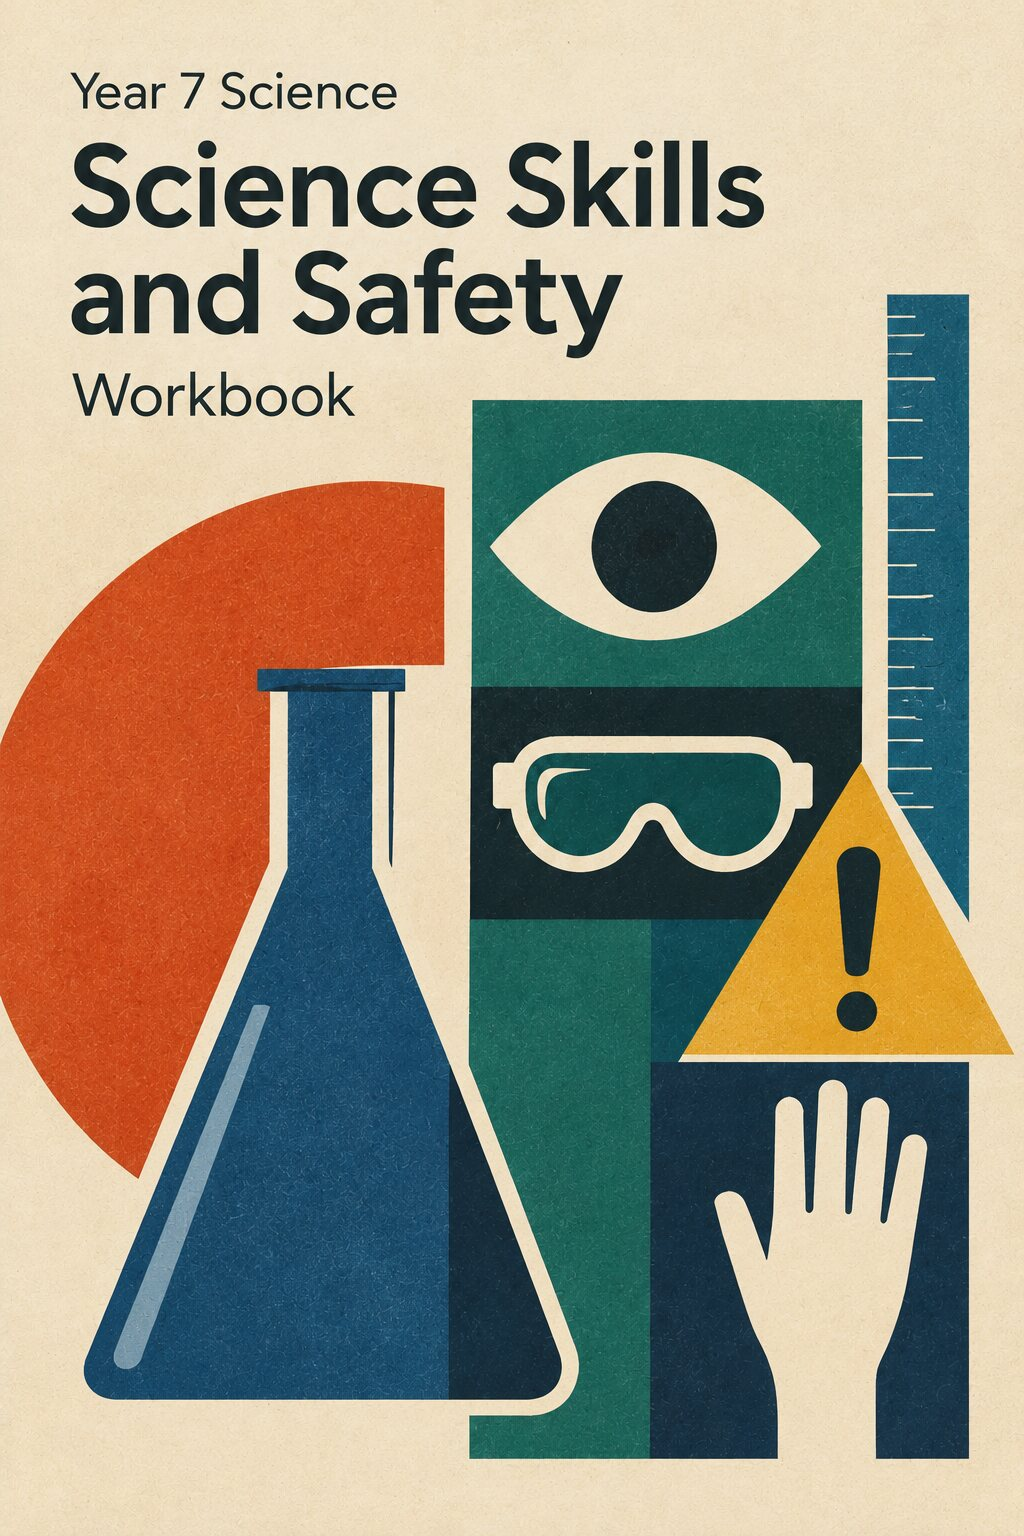
\includegraphics[width=\paperwidth]{../../covers/science-skills.jpg}};
  % Name box, top right, clear of the baked-in title ("Science Skills" ends ~140 mm in).
  \node[anchor=north east, fill=white, draw=Ink, line width=0.6pt, rounded corners=1.5mm,
        inner xsep=2.6mm, inner ysep=2.2mm, text width=40mm, font=\headingfont\small]
    at ([xshift=-6mm, yshift=-6mm]current page.north east)
    {\textbf{Name}\par\vspace{5mm}\hrule\vspace{2.6mm}\textbf{Class}\par\vspace{5mm}\hrule};
  % What this book is: the cover art says Workbook, so name the booklet here.
  \node[anchor=south east, fill=white, draw=Ink, line width=0.6pt, rounded corners=1.5mm,
        inner xsep=3.2mm, inner ysep=2.4mm, font=\headingfont\bfseries\large, align=right]
    at ([xshift=-6mm, yshift=8mm]current page.south east)
    {Experiment Booklet\\[-1pt]{\normalfont\headingfont\small Experiments 1--3}};
\end{tikzpicture}
\mbox{}
\clearpage

% ---- Inside cover ---------------------------------------------------------
\thispagestyle{plain}
{\headingfont\bfseries\fontsize{26}{30}\selectfont Science Skills and Safety}\par\vspace{1mm}
{\headingfont\Large Experiment Booklet \textbullet\ Year 7}\par\vspace{1mm}
{\small\itshape VC 2.0: VC2S8I01--I08 \textbullet\ VC2S8H01}\par\vspace{6mm}
\renewcommand{\arraystretch}{2.2}
\begin{tabular}{@{}l p{130mm}@{}}
\textbf{Name} & \hrulefill \\ \textbf{Class} & \hrulefill \\ \textbf{Teacher} & \hrulefill \\ \textbf{Lab group} & \hrulefill \\
\end{tabular}
\renewcommand{\arraystretch}{1}

\begin{countrybox}{Acknowledgement of Country}
This booklet was created on the unceded Country of the Wurundjeri Woi-wurrung people of the Kulin Nation. We acknowledge Elders past, present and emerging. Aboriginal and Torres Strait Islander peoples have observed, tested and passed on knowledge of Country for tens of thousands of years: science in the way this booklet teaches it, by careful observation, measurement and sharing what was found.
\end{countrybox}

\begin{infobox}{How this booklet works}
This booklet holds every experiment in the unit. Bring it to every practical lesson. Each experiment opens with its key vocabulary, learning intentions and skills focus, then runs \emph{Technique} $\rightarrow$ \emph{Plan and safety} $\rightarrow$ \emph{Method} $\rightarrow$ \emph{Results} $\rightarrow$ \emph{Analysis and evaluation} $\rightarrow$ \emph{Skill check}. Each kind of box has its own frame and mark:\par\smallskip
\renewcommand{\arraystretch}{1.35}
\begin{tabular}{@{}p{32mm}l@{}}
\textbf{Technique} \tagicon{\icokey} & How to do it properly (thin frame) \\
\textbf{I do} \tagicon{\icodots{1}} & Your teacher works an example through --- you follow (solid frame) \\
\textbf{We do} \tagicon{\icodots{2}} & You try one together, with help (dashed frame) \\
\textbf{You do} \tagicon{\icodots{3}} & On your own: check your understanding (heavy frame) \\
\textbf{Going further} \tagicon{\icoup} & Above level: Year 8 extension (double frame) \\
\textbf{Skills focus} \tagicon{\icoskill} & The science skills the experiment builds \\
\end{tabular}

\smallskip
Every skill comes from the faculty \textbf{Science Skills} list (the toolkit on page \pageref{sec:toolkit}). A skill always carries the same code, for example \sk{PC4} or \sk{PA1}, so you can follow it from this unit into every other unit this year.
\end{infobox}

\clearpage
{\headingfont\bfseries\LARGE Contents}\par\vspace{1mm}\noindent\rule{\linewidth}{0.6pt}\par\vspace{2mm}
\begin{ctab}
\renewcommand{\arraystretch}{1.5}
\begin{tabular}{|L{2.8cm}|L{10.2cm}|C{1.6cm}|}
  \hline\thead{Section} & \thead{Title} & \thead{Page} \\ \hline
  Skills & \hyperlink{toolkit}{The Science Skills toolkit} & \hyperlink{toolkit}{\pageref{sec:toolkit}} \\ \hline
  Skills & \hyperlink{tracker}{My skills tracker} & \hyperlink{tracker}{\pageref{sec:tracker}} \\ \hline
  Safety & \hyperlink{contract}{Lab safety contract (Lesson 5)} & \hyperlink{contract}{\pageref{sec:contract}} \\ \hline
  Experiment 1 & \hyperlink{exp.1}{Exploring the Lab (Lesson 2)} & \hyperlink{exp.1}{\pageref{sec:1}} \\ \hline
  Experiment 2 & \hyperlink{exp.2}{Measuring Mass and Volume (Lesson 3)} & \hyperlink{exp.2}{\pageref{sec:2}} \\ \hline
  Experiment 3 & \hyperlink{exp.3}{Measuring Temperature and Time (Lesson 6)} & \hyperlink{exp.3}{\pageref{sec:3}} \\ \hline
  Glossary & \hyperlink{glossary}{Key vocabulary, with the page each word first appears on} & \hyperlink{glossary}{\pageref{sec:glossary}} \\ \hline
\end{tabular}
\end{ctab}

% ══════════════════════════════════════════════════════════════════════════════
%  THE SCIENCE SKILLS TOOLKIT — faculty continuum, Years 7–8 column
% ══════════════════════════════════════════════════════════════════════════════
\clearpage
\hypertarget{toolkit}{}\pdfbookmark[1]{The Science Skills toolkit}{toolkitbm}
\markboth{The Science Skills toolkit}{}{\headingfont\bfseries\LARGE The Science Skills toolkit}\label{sec:toolkit}\par\vspace{1mm}\noindent\rule{\linewidth}{0.6pt}\par
These are the skills scientists use in every investigation. They come from the Science Inquiry strand of the Victorian Curriculum, grouped the way our faculty teaches them. Each experiment in this booklet tells you which skills it builds.

\newcommand{\tkhead}[2]{\multicolumn{3}{|l|}{\cellcolor{black!10}\rule{0pt}{4.6mm}\headingfont\bfseries #2} \\ \hline}
\newcommand{\tkrow}[1]{\skc{#1}\enspace{\small\bfseries\skname{#1}} & \skdesc{#1} & {\small\skcode{#1}} \\ \hline}
\renewcommand{\arraystretch}{1.35}
\begin{ctab}
\begin{longtable}{|W{5.0cm}|W{9.0cm}|Z{1.7cm}|}
  \hline\thead{Skill} & \thead{What it means} & \thead{Code} \\ \hline
  \endhead
  \tkhead{Teal}{Questioning and predicting}
  \tkrow{QP1}
  \tkrow{QP2}
  \tkhead{Blue}{Planning and conducting}
  \tkrow{PC1}
  \tkrow{PC2}
  \tkrow{PC3}
  \tkrow{PC4}
  \tkrow{PC5}
  \tkrow{PC6}
  \tkrow{PC7}
  \tkrow{PC8}
  \tkhead{GoldDark}{Processing, modelling and analysing}
  \tkrow{PA1}
  \tkrow{PA2}
  \tkrow{PA3}
  \tkrow{PA4}
  \tkrow{PA5}
  \tkrow{PA6}
  \tkrow{PA7}
  \tkrow{PA8}
  \tkhead{OrangeDark}{Evaluating}
  \tkrow{EV1}
  \tkrow{EV2}
  \tkrow{EV3}
  \tkrow{EV4}
  \tkrow{EV5}
  \tkhead{PurpleDark}{Communicating}
  \tkrow{CO1}
  \tkrow{CO2}
\end{longtable}
\end{ctab}
\renewcommand{\arraystretch}{1}

\begin{infobox}{Writing like a scientist \textbar\ CO1 \skname{CO1}}
Scientists write in the \textbf{third person}: say what was done, not who did it. Write \emph{``The water was heated for 10 minutes''}, not \emph{``I heated the water for 10 minutes''}. Keep sentences short, spell scientific words correctly, and always give a unit with a measurement.
\end{infobox}

% ══════════════════════════════════════════════════════════════════════════════
%  SKILLS TRACKER
% ══════════════════════════════════════════════════════════════════════════════
\clearpage
\hypertarget{tracker}{}\pdfbookmark[1]{My skills tracker}{trackerbm}
\markboth{My skills tracker}{}{\headingfont\bfseries\LARGE My skills tracker}\label{sec:tracker}\par\vspace{1mm}\noindent\rule{\linewidth}{0.6pt}\par
A dot \textbullet{} shows the experiments that build each skill. After each experiment, write how confident you are with each of its skills in its column: \textbf{1}~not yet, \textbf{2}~nearly, \textbf{3}~got it.

\newcommand{\dotc}{{\Large\textbullet}}
\newcommand{\trow}[4]{\rule[-0.36cm]{0pt}{0.92cm}\skc{#1}\enspace{\small\skname{#1}} & #2 & #3 & #4 & \\ \hline}
\begin{ctab}
\begin{tabular}{|W{5.6cm}|Z{1.8cm}|Z{1.8cm}|Z{1.8cm}|Z{2.3cm}|}
  \hline\thead{Skill} & \thead{Exp 1} & \thead{Exp 2} & \thead{Exp 3} & \thead{End of unit} \\ \hline
  \trow{QP1}{}{}{\dotc}
  \trow{PC1}{\dotc}{}{}
  \trow{PC2}{}{}{\dotc}
  \trow{PC3}{\dotc}{}{\dotc}
  \trow{PC4}{}{\dotc}{\dotc}
  \trow{PC6}{}{\dotc}{\dotc}
  \trow{PC7}{\dotc}{\dotc}{}
  \trow{PC8}{}{}{\dotc}
  \trow{PA1}{}{\dotc}{\dotc}
  \trow{PA3}{}{\dotc}{\dotc}
  \trow{PA5}{}{}{\dotc}
  \trow{PA7}{}{\dotc}{\dotc}
  \trow{EV1}{}{}{\dotc}
  \trow{EV2}{}{}{\dotc}
  \trow{EV3}{}{\dotc}{\dotc}
  \trow{CO1}{}{}{\dotc}
  \trow{CO2}{\dotc}{}{}
\end{tabular}
\end{ctab}
{\small\color{DarkGrey} Skills not in this unit (QP2, PC5, PA2, PA4, PA6, PA8, EV4, EV5) are built in the experiment booklets for later units. Graphing \sk{PA2} starts in The Particle Model, using your data from Experiment 3.}

% ══════════════════════════════════════════════════════════════════════════════
%  LAB SAFETY CONTRACT (Lesson 5)
% ══════════════════════════════════════════════════════════════════════════════
\clearpage
\hypertarget{contract}{}\pdfbookmark[1]{Lab safety contract}{contractbm}
\markboth{Lab safety contract}{}{\headingfont\bfseries\LARGE Lab safety contract}\label{sec:contract}\par\vspace{1mm}\noindent\rule{\linewidth}{0.6pt}\par
You sign this contract in Lesson 5, after the safety lesson and the safety quiz. You must pass the quiz and sign the contract before your next hands-on practical.\skr{PC3}

\begin{infobox}{In the laboratory I will \dots}
\begin{enumerate}[leftmargin=1.6em, itemsep=3pt]
  \item Enter the lab only when a teacher is present, and follow every instruction straight away.
  \item Wear safety glasses whenever chemicals, glassware or heat are being used.
  \item Tie back long hair, tuck in loose clothing and wear closed shoes.
  \item Keep bags under the bench and walkways clear.
  \item Never eat, drink or taste anything in the lab.
  \item Read the whole method before starting, and only do the experiment that has been approved.
  \item Smell a substance only by wafting it towards my nose, never by sniffing it directly.
  \item Point a heated test tube away from myself and other people.
  \item Report every spill, breakage, cut or burn to the teacher at once, however small.
  \item Put broken glass only in the broken-glass bin, never in the normal bin.
  \item Turn off the gas at the tap whenever a Bunsen burner is not being used.
  \item Clean my bench, wash my hands and return all equipment before I leave.
\end{enumerate}
\end{infobox}

\begin{scaffold}{If something goes wrong}
\textbf{Chemical in the eye:} use the eyewash station for at least 10 minutes. \quad
\textbf{Burn:} run cold water over it for 20 minutes. \quad
\textbf{Clothing on fire:} stop, drop and roll, or use the fire blanket. \quad
\textbf{Always:} tell the teacher straight away.
\end{scaffold}

\vspace{6pt}
I have read and understood the safety rules. I agree to follow them in every practical lesson. I understand that if I do not follow them I may be removed from practical work.

\vspace{12pt}
\begin{tabular}{@{}p{4.2cm}p{7cm}p{1.6cm}p{2.8cm}@{}}
  \textbf{Student signature:} & \underline{\hspace{6.6cm}} & \textbf{Date:} & \underline{\hspace{2.6cm}} \\[16pt]
  \textbf{Parent/guardian:}  & \underline{\hspace{6.6cm}} & \textbf{Date:} & \underline{\hspace{2.6cm}} \\[16pt]
  \textbf{Teacher:}          & \underline{\hspace{6.6cm}} & \textbf{Quiz:} & \underline{\hspace{2.6cm}} \\
\end{tabular}
